\documentclass[10pt,a4paper,twoside,twocolumn]{article}%ustalasz jaki typ dokumentu i właściwości

\usepackage[polish]{babel} % ustawianie języka polskiego
\usepackage[colorlinks=false,linkcolor=green,urlcolor=green,citecolor=green]{hyperref}%hiperłącza ogólnego rodzaju
\hypersetup{pdftitle=Sprawozdanie SSR}

\usepackage{pdfpages} % importowanie plików z pdfa
\usepackage{amsmath} % do wstawiania macierz itp
\usepackage{graphicx} % wstawianie zdjęć
% \usepackage[utf8]{inputenc} % niepotrzebne bo lualatex
\usepackage[T1]{fontenc} % niepotrzebne bo lualatex
\usepackage[left=1cm,right=1cm,top=1cm,bottom=2cm,
columnsep=1cm % odstęp między kolumnami
]{geometry}%marginesy

\usepackage{listings} % punktowanie
% \usepackage{indentfirst} % dawanie akapitu na początku
\usepackage{caption} % podpisy
\usepackage{subcaption} % podpisy do subfigure
\usepackage{siunitx} % jednostki si
\usepackage{minted} % ładne kody naprzyklad matlaba
\setminted{linenos=true,frame=single,breaklines=true,breaksymbolleft=,style=vs}

\usepackage{textcase}

\usepackage[polish,nameinlink]{cleveref} % dobre prefiksy przed etykietą i język
\usepackage{cprotect}

\usepackage{fontspec}
% \setmainfont[Ligatures=TeX]{Georgia}
% \setsansfont[Ligatures=TeX]{Arial}
\usepackage{parskip} % usunięcie tab na początku akapitu
\usepackage{newfloat} % aby można było ładnie wstawić elementy typu zdjecie, kod itp

%%% rysowanie wykresów %%% ale w ciul to trudne więc app.diagrams.net
\usepackage{tikz}
\usetikzlibrary{shapes.geometric, arrows, positioning}

% % % SVG import
\usepackage{svg}
\usepackage{import}
\usepackage{xifthen}
\usepackage{transparent}

% \usepackage{mdframed} % ramki
\usepackage[framemethod=TikZ]{mdframed}
\mdfsetup{%
middlelinecolor=red,
middlelinewidth=1pt,
   backgroundcolor=gray!20,
   roundcorner=10pt}

\usepackage{enumitem} % podpunkty customowe

\usepackage{pgfplots}[compat=1.18] % wykresy


%%%%%%%%%%%%%% koniec pakietów %%%%%%%%%%%%%%%%%%%%%%%%%%%

\boldmath%pogrubiona matma

\title{Fajny ten tytuł}%tytuł
\date{\today}%%data
\author{Janusz Chmaruk}%autor
\setcounter{secnumdepth}{3}%głębokość liczenia roździałów

% PRZYKŁAD LICZNIKA ZADAŃ
\newcounter{zadanie}
\newenvironment{zadanie}[1][]{
   \refstepcounter{zadanie}
   \subsection*{Zadanie \thezadanie#1}
   \addcontentsline{toc}{subsection}{Zadanie \thezadanie#1} % dodanie do spisu treści
}{}


% DŁUGIE LISTINGI
\newenvironment{longlisting}{\captionsetup{type=listing}}{}

%%%%%%%%%%%%%%%%%%%%%%%%%%%%%%%%%%%%%%%%%%%%%%%%%%%%%%%%%%%%%%%
%%%%%%%%%%%%%%%%%%%%%%%%%%%%%%%%%%%%%%%%%%%%%%%%%%%%%%%%%%%%%%%
%%%%%%% TU SIE ZACZYNA PISANIE PLIKU %%%%%%%%%%%%%%%%%%%%%%%%%%
%%%%%%%%%%%%%%%%%%%%%%%%%%%%%%%%%%%%%%%%%%%%%%%%%%%%%%%%%%%%%%%
%%%%%%%%%%%%%%%%%%%%%%%%%%%%%%%%%%%%%%%%%%%%%%%%%%%%%%%%%%%%%%%

\begin{document}%zaczyna się dokument

% \null%
% 
\includepdf[pages={1}]{Szablon_Projektu.pdf}
\clearpage%następna strona ogółem

\tableofcontents%spis treści
% \clearpage


\begin{zadanie}
    Omówić zasadę doboru częstotliwości próbkowania; Zilustrować na przykładzie sygnału $t=0:1$; $y=sin(2*\pi*3*t)$;
    narysuj sygnał i widmo sygnału po spróbkowaniu. \textbf{4p}
\end{zadanie}\\

    \begin{mdframed}[backgroundcolor=gray!20,]
        Częstość próbkowania musi być większa niż dwukrotność częstotliwości najwyższej składowej sygnału.
        $$f_{max} = 3$$
        $$f_{\text{próbkowania}} > 2*f_{max}$$
        $$f_{\text{próbkowania}} > 6$$

        \begin{tikzpicture}
            \centering
            \begin{axis}[
                xlabel={$t$},
                ylabel={$y$},
                xmin=0, xmax=1,
                ymin=-1, ymax=1,
                xtick={0,0.1,0.2,...,1}, % Ustalanie kroków próbkowania
                domain=0:1,
                samples=100
            ]
            \addplot[blue] {sin(deg(6*x))};
            \addplot[red, only marks, mark=*, mark size=1.5pt, samples at={0,0.1,0.2,...,1}] {sin(deg(6*x))};
            \end{axis}
        \end{tikzpicture}
    \end{mdframed}

\begin{zadanie}
    Dla filtra o następującej strukturze:
    \begin{figure}[H]
        \centering
        \includegraphics[width=1\linewidth]{Diagram bez tytułu.drawio.pdf}
    \end{figure}
    \begin{enumerate}[label=\alph*)]
        \item podać rodzaj(SOI/NOI) i rząd filtra; \textbf{1p}
        \item wyznaczyć odpowiedź impulsową; \textbf{1p}
        \item narysować odpowiedź na sygnał: $x(k) = \delta (k-1)-\delta(k −3)$; \textbf{4p}
        \item wyznaczyć równanie różnicowe opisujące filtr; \textbf{2p}
        \item wyznaczyć transmitancję filtra; wyznaczyć charakterystykę częstotliwościową filtra; \textbf{2p}
        \item określić stabilność filtra; \textbf{1p}
    \end{enumerate}
\end{zadanie}

\begin{mdframed}[backgroundcolor=gray!20,roundcorner=7pt]
    \begin{enumerate}[label=\alph*)]
        \item Filtr jest SOI, rząd filtra to 3. 
        \item odpowiedź impulsowa to: $h(k) = 2*\delta(k) + (-1)*\delta(k-1) + 3*\delta(k-3)$ 
        \item Odpowiedź sygnału:
            \begin{table}[H]
                \centering
                \begin{tabular}{|c|c|}
                    \hline
                    k & y(k) \\ \hline
                    0 & 0 \\ \hline
                    1 & 2 \\ \hline
                    2 & -1 \\ \hline
                    3 & -2 \\ \hline
                    4 & 4 \\ \hline
                    5 & 0 \\ \hline
                    6 & -3 \\ \hline
                    7 & 0 \\ \hline
                \end{tabular}
            \end{table}
        \item Równanie różnicowe:$$2x(k)-1x(k-1)+3x(k-3)$$
            
        \item Transmitacja filtra:$$y(k) = 2 + (-1)z^{-1} + 3z^{-3}$$
            Charakterystyka częstotliwościowa filtra:$$$$
            
        \item Filtr jest stabilny
    \end{enumerate}
\end{mdframed}
\begin{figure}[H]
    \centering
    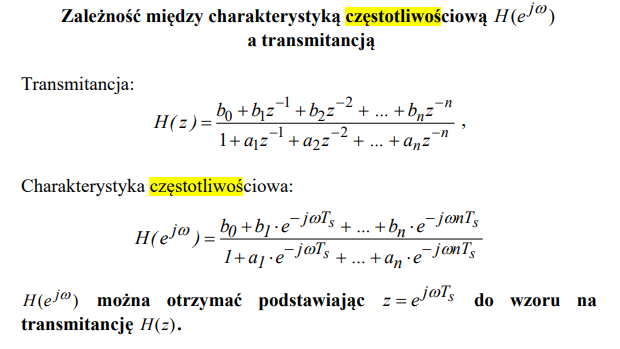
\includegraphics[width=1\linewidth]{image.png}
\end{figure}



\begin{zadanie}
    Na przykładzie filtru dolnoprzepustowego omówić podstawowe cechy ciągłego filtru Czebyszewa. Porównać charakterystyki częstotliwościowe filtru analogowego i cyfrowego. \textbf{3p}
\end{zadanie}

\begin{mdframed}[backgroundcolor=gray!20,]
    
    Charakterystyka amplitudowa flitru jest równomiernie zafalowana w paśmie przepustowym oraz
monotoniczna w zaporowym lub charakterystyka amplitudowa monotoniczna w paśmie
przepustowym oraz równomiernie zafalowana w zaporowym.\\

Filtr Czebyszewa zwykle ma niższy stopień niż filtr Butterwortha przy tych samych
wymaganiach (dzięki bardziej stromej charakterystyce w paśmie przejściowym).\\

Porównanie:
% \begin{itemize}
%     \item Porównując filtry analogowe i cyfrowe, istnieją pewne kluczowe różnice:

%     \item Dokładność: Filtry cyfrowe mogą być bardziej dokładne niż ich odpowiedniki analogowe, ponieważ nie są podatne na wpływ szumów i zakłóceń analogowych.
    
%     \item Złożoność realizacji: Filtry cyfrowe mogą być trudniejsze do zrealizowania w praktyce, ponieważ wymagają skomplikowanych układów cyfrowych i procesorów sygnałowych.
    
%     \item Zakres częstotliwości: Filtry analogowe mogą pracować z sygnałami o wyższych częstotliwościach niż filtry cyfrowe, które są ograniczone przez częstotliwość próbkowania.
    
%     \item Zastosowania: Filtry analogowe są często stosowane w radiotechnice i innych aplikacjach, które wymagają przetwarzania sygnałów w czasie rzeczywistym. Filtry cyfrowe są często stosowane w aplikacjach, które wymagają wysokiej dokładności i elastyczności, takich jak przetwarzanie obrazów i dźwięku.
% \end{itemize}
Zalety transformacji biliniowej (z analogowego na cyfrowy):
\begin{itemize}
    \item zachowana stabilność,
    \item brak efektu nakładania się widm.
\end{itemize}

Wady transformacji biliniowej:
\begin{itemize}
    \item zniekształcenie osi częstotliwości.
\end{itemize}
    
\textbf{Chat GPT:}\\
Filtry Czebyszewa są rodzajem filtrów, które zapewniają optymalizację między
szerokością pasma przenoszenia a tłumieniem w paśmie zaporowym. Są one nazwane
na cześć rosyjskiego matematyka Pafnutiego Czebyszewa. Podstawowe cechy filtrów
Czebyszewa to:

Ryple (fale) w paśmie przenoszenia: Filtry Czebyszewa typu 1 mają
charakterystyczną cechę, która polega na tym, że mają ryple (fluktuacje) w
paśmie przenoszenia. Wielkość tych rypli jest jednym z parametrów projektowania
filtru. Większe ryple prowadzą do szybszego tłumienia poza paśmie przenoszenia,
ale kosztem większych zniekształceń w paśmie przenoszenia.

Szybkość tłumienia: Filtry Czebyszewa są znane z tego, że zapewniają szybkie
tłumienie poza paśmie przenoszenia. W porównaniu do innych typów filtrów, takich
jak filtry Butterwortha, filtry Czebyszewa mogą osiągnąć tłumienie o określonej
wielkości przy mniejszej liczbie stopni (rzędu filtru).

Optymalizacja Czebyszewa: Filtry Czebyszewa są zaprojektowane tak, aby
minimalizować maksymalne odchylenie od idealnej charakterystyki w określonym
zakresie częstotliwości. Oznacza to, że filtr Czebyszewa zapewnia optymalne
rozwiązanie problemu Czebyszewa.

Charakterystyki częstotliwościowe filtrów analogowych i cyfrowych różnią się
pod wieloma względami:

Zakres częstotliwości: Filtry analogowe działają na sygnałach ciągłych i mogą
przetwarzać sygnały o dowolnej częstotliwości, ograniczonej tylko przez
charakterystyki sprzętowe. Z drugiej strony, filtry cyfrowe działają na
sygnałach dyskretnych i są ograniczone przez częstotliwość Nyquista, która jest
połową częstotliwości próbkowania.

Stabilność: Filtry analogowe mogą mieć problemy ze stabilnością, zwłaszcza dla
filtrów o wysokim rzędzie. Filtry cyfrowe są zazwyczaj bardziej stabilne,
chociaż mogą wystąpić problemy ze stabilnością w przypadku filtrów IIR.
\end{mdframed}

\begin{zadanie}
    Podać warunek liniowej fazy filtrów SOI dla N parzystego i nieparzystego i omówić jaki wpływ ma liniowa faza na filtrowany sygnał? \textbf{3p}
\end{zadanie}
\begin{mdframed}
    % Filtrowanie liniowofazowe jest możliwe, gdy odpowiedź impulsowa systemu jest symetryczna lub antysymetryczna.
    % Warunek liniowości fazy:
    % %Symetryczny (typ I i II): 
    % $h[k] = h[N - k]$ dla wszystkich $k$, gdzie $N$ to
    % rzęd filtru.

Filtr FIR (SOI) ma liniową charakterystykę fazy, gdy jest symetryczny lub
antysymetryczny, co znaczy, że jego odpowiedź impulsowa spełnia jeden z
poniższych warunków:\\
 Symetryczny (typ I i II): $h[n] = h[N - n]$ dla wszystkich $n$,
gdzie $N$ to rzęd filtru.\\
 Antysymetryczny (typ III i IV): $h[n] = -h[N - n]$ dla
wszystkich $n$. \\
Filtry FIR, które spełniają te warunki, nazywane są filtrami o
liniowej fazie.\\
 Liniowa faza jest pożądana, ponieważ utrzymuje relacje fazowe
pomiędzy różnymi składowymi częstotliwościowymi sygnału. Innymi słowy, wszystkie
składowe częstotliwościowe sygnału są przesunięte w czasie o tę samą ilość, co
oznacza, że kształt sygnału jest zachowany po filtracji. To jest szczególnie
istotne w wielu zastosowaniach, takich jak przetwarzanie dźwięku i obrazu, gdzie
zachowanie kształtu sygnału jest kluczowe. W przeciwnym razie, jeśli faza nie
jest liniowa, różne składowe częstotliwościowe mogą być przesunięte o różne
ilości, co prowadzi do zniekształceń, takich jak ``rozmycie'' sygnału.\\
$$n=k$$
    
\end{mdframed}
\begin{zadanie}{}
    Podać definicje funkcji autokorelacji R, funkcji autokowariancji C ergodycznego \textbf{1p}, stacjonarnego szeregu losowego X. Wyznaczyć wartość średnią tego procesu oraz funkcję autokorelacji z dostępnej realizacji czasowej $x = [3,5,2,4,2]$ tego procesu losowego. Narysować tę funkcję autokorelacji. \textbf{3p}
    Wyznaczyć macierz autokorelacji R. \textbf{2p}
\end{zadanie}

\begin{mdframed}
    Funkcja autokorelacji jest miarą podobieństwa między wartością sygnału w danym
    czasie a wartościami sygnału w innych czasach. Definiuje ona zależność między
    dwiema kolejnymi wartościami sygnału i mierzy, jak bardzo te wartości są
    skorelowane. Funkcja autokowariancji mierzy kowariancję między dwiema
    wartościami sygnału w różnych momentach czasowych. Jest to szczególny przypadek
    funkcji autokorelacji, w którym oczekiwana wartość sygnału jest równa zero.
    Szereg losowy X jest nazywany stacjonarnym jeśli jego średnia nie zależy od
    czasu oraz funkcja autokorelacji zależy tylko od różnicy między czasami, a nie
    od samych czasów. Stacjonarny szereg losowy ergodyczny spełnia dodatkowo warunek,
    że wartości średnie uzyskane na podstawie jednych realizacji są reprezentatywne
    dla wartości średnich uzyskanych na podstawie innych realizacji.
    
    $$(3+5+2+4+2)/5 = 3.2$$
    
    $$R(0) = (1/5) * [(3-3.2)^2 + (5-3.2)^2 + (2-3.2)^2$$$$ + (4-3.2)^2 + (2-3.2)^2] = 1.76$$
    
    $$R(1) = (1/4) * [(3-3.2)(5-3.2) + (5-3.2)(2-3.2)$$$$ + (2-3.2)(4-3.2) + (4-3.2)(2-3.2)] = -0.8$$
    
    $$R(2) = (1/3) * [(3-3.2)(2-3.2) + (5-3.2)(4-3.2)$$$$ + (2-3.2)(2-3.2)] = 0$$
    
    $$R(3) = (1/2) [(3-3.2)(4-3.2)$$$$ + (5-3.2)(2-3.2)] = -0.8$$
    
    $$R(4) = (1/1) * [(3-3.2)*(2-3.2)] = 0$$

    $$R = \begin{bmatrix}
        1.76 & -0.8 & 0 & -0.8 & 0 \\
        -0.8 & 1.76 & -0.8 & 0 & -0.8 \\
        0 & -0.8 & 1.76 & -0.8 & 0 \\
        -0.8 & 0 & -0.8 & 1.76 & -0.8 \\
        0 & -0.8 & 0 & -0.8 & 1.76
        \end{bmatrix}$$
        

\end{mdframed}

\begin{zadanie}{}
Filtr Wienera zazwyczaj jest filtrem SOI i pracuje w strukturze


    $$y(n)=\sum_{k=0}^{M}h(k)x(n-k)=h^{T}x(n)$$
    $$h=[h_0,h_1,...,h_M]^{T}$$
    $$x(n)=[x(n),x(n-1),x(n-2)\dots,x(n-M)]^T$$

    \begin{figure}[H]
        \centering
        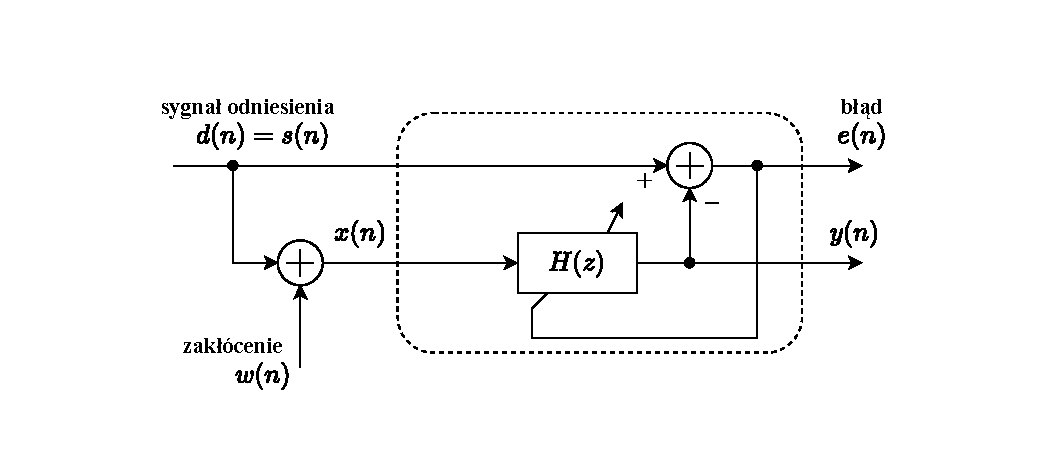
\includegraphics[width=1\linewidth]{2.drawio.pdf}
    \end{figure}
Podać wskaźnik jakości optymalizacji, który prowadzi do uzyskania optymalnego zbioru współczynników filtru \textbf{h}. Podać rozwiązanie problemu optymalizacji w postaci macierzowo-wektorowego równania Wienera-Hopfa. \textbf{4p}
\end{zadanie}


\begin{mdframed}
    Filtr Wienera jest zaprojektowany do minimalizacji średniej kwadratowej
    błędu (MSE - mean square error) między sygnałem oczekiwanym a rzeczywistym
    sygnałem wyjściowym. MSE jest wskaźnikiem jakości optymalizacji, który jest
    zdefiniowany jako: $E{(d(n) - y(n))^2}$ \\
    gdzie:\\
    $E\{\dots\}$ oznacza wartość oczekiwaną (średnią),\\ 
    $d(n)$ to oczekiwany (docelowy) sygnał,\\
    $y(n)$ to rzeczywisty sygnał wyjściowy.\\

    Równanie Wienera-Hopfa Równanie Wienera-Hopfa to kluczowe równanie w teorii filtrów Wienera, które pozwala
    na wyznaczenie optymalnych współczynników filtru. W przypadku liniowego,
    czasowo niezmiennego filtru Wienera, równanie Wienera-Hopfa ma postać: $R_{xx}
    * h = r_{dx}$ gdzie:\\
     $R_{xx}$ to autokorelacyjna macierz sygnału wejściowego $x$,\\
     $h$ to wektor współczynników filtru, który chcemy optymalizować,\\
      $r_{dx}$ to wektor
    krzyżowej funkcji korelacji między sygnałem wejściowym x a sygnałem
    docelowym d.\\

     Rozwiązaniem tego równania jest wektor optymalnych
    współczynników filtru h. Możemy to zrobić, na przykład, za pomocą metody
    odwracania macierzy lub innych technik rozwiązywania równań liniowych. \\

\end{mdframed}

\end{document}